\section{Design decisions}
During the design of the project, several design decisions were made, they are listed here.
\begin{itemize}
\item Petrol cards
\begin{itemize}
\item PIN code is used for authenticating the card owner to the terminals.
\item Public Key Infrastructure (PKI) is used for authentication, encryption and signatures of messages.
\item The petrol card will have an initial balance of zero once a car owner receives the petrol card. 
%\item All communications between petrol card and terminal are encrypted \& signed with a symmetric key. %except for the first communication of the certificate by either one party.
\item A symmetric key is used to secure communication between the petrol card and the terminal.
\item Petrol cards will have their own certificates and key material that will be initialised by the IT.
\end{itemize}

\item Terminal
\begin{itemize}
\item The IT will set the initial balance to zero.
\item The PIN codes will be set by the IT.
\item The CT will relay the signed allowance by the back end to the petrol card.
\item A symmetric key is used to secure communication between the terminal and back-end.
\item The petrol allowance on the petrol card can only be charged once a month.
\item The CT can see the petrol balance stored on the petrol card after the CT has authenticated itself to the petrol card.
\item The card owner will have to specify the required amount of petrol that he wishes to pump at the PT. In a previous design we planned on subtracting all balance from the petrol card. 
\end{itemize}


%\item Will ask for amount of fuel that is to be released. Card holder knows how much fuel is going to be used. Once entered, the card holder does not get rest of allowance back. So the pump terminal is not able to write allowance to the card.



%will the correct amount of used petrol Card owner will have to insert the petrol card into the petrol terminal for the whole transaction. The petrol terminal will receive the current petrol allowance on the card, the flow of petrol will be terminated if it reaches this number. If the petrol allowance is removed before the transaction is complete, the full petrol allowance will be removed upon the next presentation at a charging or petrol terminal. 

% until the fuel amount is chosen by the card owner. Petrol allowance on the card is provided to terminal, if the card is removed or this amount has been reached, the flow of petrol will be terminated. If the petrol card is removed during this moment, all petrol allowance will be removed from the card ???
%petrol allowance on the card will be decreased before its added to petrol terminal



\item Back-end
\begin{itemize}
\item The back-end will sign and send the latest version of the CRL to the terminals
	%\item Will have a signed list of blocked petrol cards that are issued to the terminals.
%	\item Will have a list of all ID numbers belonging to each petrol card and terminal
%	\item Will have a sub-CA certificate, the utmost level in the certificate chain apart from the main CA.
%	\item The main CA certificate will only be used to sign and revoke sub-CA certificates
\end{itemize}
\end{itemize}

%\section{Overall design}
\subsection{PIN codes}
The user will have to enter a PIN code on the terminal numpad to verify ownership of the petrol card to the terminal. The terminal will send the PIN signed by its private key with the plain text of the PIN to the petrol card through the mutually authenticated encrypted channel. By which the petrol card will reply with whether the PIN number is correct or not.

\subsection{Cryptography and PKI}
PKI is used to maintain and generate certificates. The back-end will operate as CA. We planned on creating a sub-CA to sign all terminal and petrol card certificates, but due to time constraints this was not possible. In the current situation the certificate of the main CA will be stored on a newly personalised petrol card. The back-end, terminals and petrol cards will all have a RSA-1024 bit keypair. While this is not secure for real-world purposes, for testing and petrol card limitations, this will have to do. The petrol card and terminals will receive a timestamp of the last update of certificate revocation list which is signed by the main CA certificate. This way it can be verified if the provided revocation list is recent. Each terminal will have the same setup: main CA certificate, its RSA keypair, and signed timestamp of the last updated certificate revocation list. \\

The CA certificate on each device is used to verify the validity and authenticity of each certificate during communication. Each end point, i.e petrol card and terminal, will verify the certificate of the other end point it is connecting to. In case the CA is notified of abuse or a breach, the certificate belonging to the end point will only be usable for 24 hours until the revocation list has been pushed to the end points. % At this point it is important to verify if the certificate has not been revoked by the CA. This way when the CA has been notified of abuse or breach in one of the end points, it will only take 24 hours for each end point to know of the revocation of a particular certificate. \\

Public and private keys in each end point will be used in conjunction with the CA certificate to mutually authenticate between each other. It is also used to negotiate a SK and also to provide integrity of the message by signing them.

 %A certificate consisting of a public and private key will be first created on the back-end (the overall system acting as the Certificate Authority). 

%\subsection{Public and Private keys in terminals/petrol cards}



\subsection{Protocol Descriptions}
\subsubsection{Mutual Authentication}
First the terminal sends a command APDU to enable the correct applet from the petrol card for the petrol rationing system. After that the terminal sends its certificate and public key to the petrol card. The petrol card verifies the certificate of the terminal and chooses a SK for encrypted communication. The petrol card signs its identification number with its private key, encrypts that signature and its own certificate with the SK. Then it sends the encrypted signature and certificate together with the SK encrypted by the public key of the terminal. Once the terminal receives the certificate of the petrol card, it verifies it. It then signs its own signature with its private key and combines this with a signed version of the identification number, encrypts them both with the SK and sends it to the petrol card.
\\

\begin{equation}\nonumber
\begin{split} 
T \to PC &: \text{commandAPDU to enable applet.}\\
T \to PC &: certificate_{T}, pub_{T}\\ 
PC &: \text{Verify}(certificate_{T}) \text{and choose SK}\\
PC \to T &: ENC_{SK}\{SIG[ID_{PC}]_{priv_{PC}}, certificate_{PC}\},  [SK]_{pub_T}\\
T&: \text{Verify}(certificate_{PC})\\
T \to PC &: ENC_{SK}\{SIG[ID_{T}]_{priv_T}, ID_{T}\} \\ 
\end{split} 
\end{equation}
and now we have a encrypted channel between a terminal and a petrol card.

\subsubsection{Certificate Validity Request}
After mutual authentication has been done, the petrol card will request the certificate revocation list from the terminal, who already has access the latest revocation list from the back-end. The revocation list is signed by the back-end. 

\begin{equation}\nonumber
\begin{split}
PC \to T &: [CVR + pub_{PC}]_{pub_{BE}}\\
T \to PC &: [SIG[VTS, TS, Certs]_{priv_{BE}}, VTS, TS, Certs]_{pub_{PC}}
\end{split} 
\end{equation}

\subsubsection{PIN validation and authentication of card owner}
After mutual authentication has been done, the terminal receives a PIN on the numpad from the card owner, signs the PIN and send the encryption of the signature with the plaintext PIN number to the petrol card. Once the petrol card receives the PIN number, returns the encrypted and signed boolean value (True/False) to the terminal after it verifies the PIN number. \\

PIN validation and authentication of card owner guarantees security requirement 1(d).

\begin{equation}\nonumber
\begin{split}
T \to PC&: ENC_{SK}\{SIG[PIN]_{priv_T}, PIN\}\\
PC \to T&: ENC_{SK}\{SIG[PIN_{AUTH}]_{priv_{PC}}, PIN_{AUTH}\}
\end{split} 
\end{equation}

\subsubsection{Getting petrol from the petrol terminal}
After mutual authentication and authentication of the card owner, the petrol card can send its current balance to the petrol terminal for getting petrol. The card owner will have to specify the amount of petrol he wishes to subtract from his balance. The PT will verify if this is possible and subtract this amount from the petrol card. After the transaction has been verified the PT will write a log entry with the time, identification number of the petrol card, balance and amount of  petrol that was pumped. If a card tear occurs the specified amount of petrol will be reduced from the petrol cards balance. We planned on adding something to this log that is signed by the card (such as balance and/or timestamp), however due to time constraints this was not implemented.  %Then, the terminal writes a balance of zero to the petrol card for cases where the card was removed mid transaction. Once the petrol has been pumped and the user successfully terminates the program, the terminal writes a new balance after deducting the pumped petrol amount from the initial balance sent by the card, to the card. And immediately after that the terminal logs the time, identification number, balance and the amount of petrol pumped by the user.

The terminal logging the timestamp, identification number and the balance before the petrol being pumped guarantees security requirement 5(b).

\begin{equation}\nonumber
\begin{split}
PC \to T&: ENC_{SK}\{SIG[B]_{priv_{PC}}, B\}\\
T&: \text{Log}(TS, ID_{PC}, B, SIG[TS, ID_{PC}, B]_{priv_T}) \\
T \to PC&: ENC_{SK}\{SIG[BZ]_{priv_T}, BZ\}\\
T&: \text{Calc}(B = B - UB)\\
T \to PC&: ENC_{SK}\{SIG[B]_{priv_T}, B\}\\
T&: \text{Log}(TS, ID_{PC}, B, UB, SIG[TS, ID_{PC}, B, UB]_{priv_T})
\end{split} 
\end{equation}


\subsubsection{Charging petrol allowance to the petrol card}
After mutual authentication, PIN validation and authentication of card owner
has been done, the petrol card can ask the charging terminal to charge its
allowed monthly petrol balance. Then the terminal starts a mutually
authenticated encrypted channel between itself and the back-end to get the monthly petrol allowance, and then
writes those values back to the petrol card.\\

The terminal starting a mutually authenticated encrypted channel with the back-end to get the monthly petrol allowance guarantees security requirement 1(e) \& 3(c).\\

The terminal logging the timestamp, identity number and the balance being written to the petrol card guarantees security requirement 6(a).

\begin{equation}\nonumber
\begin{split}
PC \to T&: \text{request APDU to initiate charging monthly allowance} \\
T&: \text{requests monthly allowance from back-end through the encrypted channel} \\
T&: \text{Log}(TS, ID_{PC}, B, SIG[TS, ID_{PC}, B]_{priv_T}) \\
T \to PC&: ENC_{SK}\{SIG[B,TS]_{priv_{BE}}, B, TS\}
\end{split} 
\end{equation}

\subsubsection{Invalidating petrol cards}
Petrol cards are invalidated by the back-end by means of revoking the certificate, which will be added to the revocation list. Cards can be added to the revocation list if the certificate is valid, if authentication of the user failed (incorrect PIN entry for three times), or any other suspicious behaviour \textcolor{red}{Possible other scenarios..}.


\textcolor{red}{TODO: explain how persistant and transient states are realised in the code }
\begin{figure}[!ht]
  \centering
    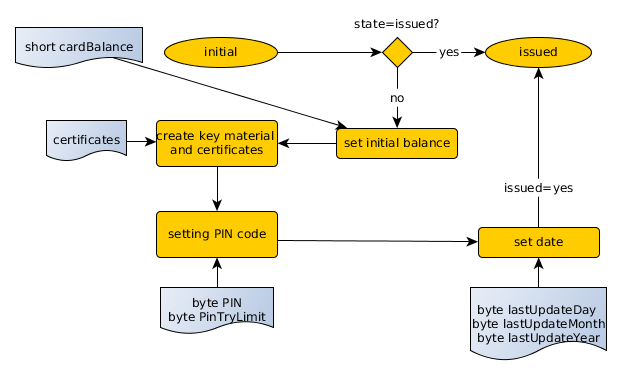
\includegraphics[width=0.8\textwidth]{persistant}
      \caption{The persistant states of the petrol card.}
\end{figure}

\begin{figure}[!ht]
  \centering
    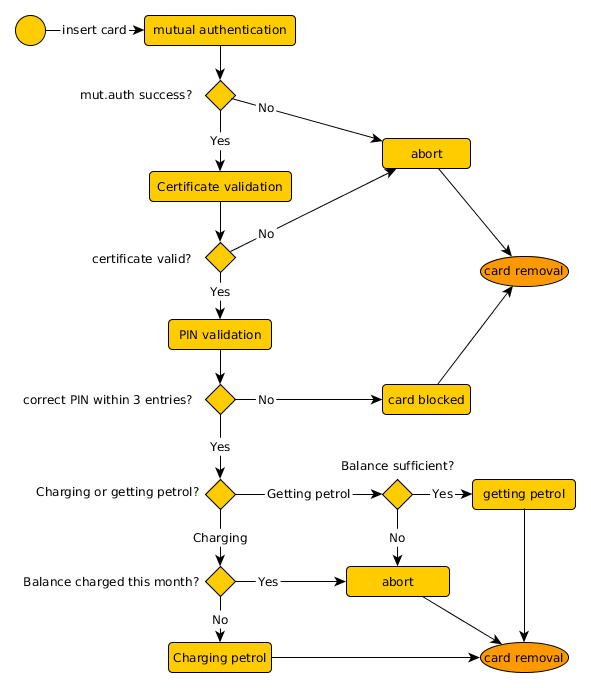
\includegraphics[width=0.8\textwidth]{transient}
      \caption{The transient states of the petrol card.}
\end{figure}